\documentclass[a4paper,oneside]{article}
\usepackage[utf8]{inputenc}
\usepackage{underscore}
\usepackage{setspace}
\usepackage{indentfirst} 
\usepackage{mathtools}
\usepackage{amsfonts}
\usepackage{enumitem}
% \usepackage[standard]{ntheorem}
\usepackage{amsthm}
\usepackage{cancel}
\usepackage{amssymb}
\usepackage[left=1.4cm,right=1.4cm,
    top=2.3cm,bottom=2.3cm,bindingoffset=0cm]{geometry}
\singlespacing

\usepackage{graphicx}
\graphicspath{ {./images/} }

\usepackage{fancyhdr}
\pagestyle{fancy}

\usepackage{tikz}
\usepackage[T2A]{fontenc}
\usepackage{graphicx}
\usepackage[sort,compress]{cite}
\usepackage{amsmath}
\usepackage{amssymb}
\usepackage{amsthm}
\usepackage{fancyvrb}
\usepackage{listings}
\usepackage{listingsutf8}
\usepackage{longtable}
\usepackage{array}
\usepackage[english,russian]{babel}
\usepackage{minted}

\usepackage[colorlinks=true]{hyperref}
\usepackage{url}
\usepackage{tempora}
\newcommand{\eqdef}{\stackrel {\rm def}{=}}

\usepackage{tabularx}
\newcommand{\bydef}{\stackrel{\text{по опр.}}{\implies}} % by definition - по определению
\newcommand{\parspace}{\vspace{10pt}}

\newcommand{\logor}{\vee}
\newcommand{\logand}{\wedge}

\newcommand{\imagin}{\mathrm{Im} \,}
\newcommand{\real}{\mathrm{Re} \,}

\newcommand{\dslim}{\displaystyle\lim}
\newcommand{\dslimn}{\dslim_{n \to \infty}}

\newcommand{\prop}[1]{#1^{\text{o}}}

\newcommand{\N}{\mathbb{N}}
\newcommand{\R}{\mathbb{R}}
\newcommand{\bb}[1]{\mathbb{#1}}

\newcommand{\eps}{\varepsilon}

\newcommand{\approach}[1]{\underset{#1}{\longrightarrow}}

% \theoremstyle{break}

% --- Теорема --- %
% \newtheoremstyle{break}% name
%   {}%         Space above, empty = `usual value'
%   {}%         Space below
%   {\itshape}% Body font
%   {}%         Indent amount (empty = no indent, \parindent = para indent)
%   {\bfseries}% Thm head font
%   {.}%        Punctuation after thm head
%   {\newline}% Space after thm head: \newline = linebreak
%   {}%         Thm head spec
% \theorembodyfont{\normalfont}
% \theoremstyle{break}
\newtheorem{theorem}{Теорема}[subsection]
% --------------- %

% --- Определение --- %
% \theorembodyfont{\normalfont}
\theoremstyle{definition}
\newtheorem{definition}{Определение}[subsection]
% ------------------- %

% --- Доказательство --- %
% \theoremheaderfont{\normalfont\itshape}
% \theorembodyfont{\normalfont}
% \newtheorem*{proof}{Доказательство.}
% ---------------------- %

% --- Пример --- %
\theoremstyle{definition}
\newtheorem*{example}{Пример}
% -------------- %

% --- Следствие --- %
% Corollary
% ----------------- %

% --- Замечание --- %
% Remark
\theoremstyle{definition}
\newtheorem*{remark}{Замечание}
% ----------------- %


\begin{document}

%----------------------------------------------------------------------------------------
%	TITLE PAGE
%----------------------------------------------------------------------------------------

\begin{titlepage} % Suppresses displaying the page number on the title page and the subsequent page counts as page 1
	\newcommand{\HRule}{\rule{\linewidth}{0.5mm}} % Defines a new command for horizontal lines, change thickness here
	
	\center % Centre everything on the page
	
	%------------------------------------------------
	%	Headings
	%------------------------------------------------
	
	\textsc{\LARGE Издательство Пупы и Лупы}\\[1.5cm] % Main heading such as the name of your university/college
	
	\textsc{\Large }\\[0.5cm] % Major heading such as course name
	
	\textsc{\large }\\[0.5cm] % Minor heading such as course title
	
	%------------------------------------------------
	%	Title
	%------------------------------------------------
	
	\HRule\\[0.4cm]
	
	{\huge\bfseries Лекции по лучшему языку на планете}\\[0.4cm] % Title of your document
	
	\HRule\\[1.5cm]
	
	%------------------------------------------------
	%	Author(s)
	%------------------------------------------------
	
	\begin{minipage}{0.4\textwidth}
		\begin{flushleft}
			\large
			\textit{Автор}\\
			\textsc{Пупа} % Your name
		\end{flushleft}
	\end{minipage}
	~
	\begin{minipage}{0.4\textwidth}
		\begin{flushright}
			\large
			\textit{Редактор}\\
			\textsc{Лупа} % Supervisor's name
		\end{flushright}
	\end{minipage}
	
	% If you don't want a supervisor, uncomment the two lines below and comment the code above
	%{\large\textit{Author}}\\
	%John \textsc{Smith} % Your name
	
	%------------------------------------------------
	%	Date
	%------------------------------------------------
	
	\vfill\vfill\vfill % Position the date 3/4 down the remaining page
	
	{\large\today} % Date, change the \today to a set date if you want to be precise
	
	%------------------------------------------------
	%	Logo
	%------------------------------------------------
	
	%\vfill\vfill
	%\includegraphics[width=0.2\textwidth]{placeholder.jpg}\\[1cm] % Include a department/university logo - this will require the graphicx package
	 
	%----------------------------------------------------------------------------------------
	
	\vfill % Push the date up 1/4 of the remaining page
	
\end{titlepage}

%----------------------------------------------------------------------------------------

\section{Теория множеств}

\subsection{Множества и отношения между ними}

Множество "--- совокупность различаемых объектов.
Объекты называются его элементами.

Два множества равны ($A = B$), если:

\begin{equation*}
     \forall x: (x \in A \Leftrightarrow x \in B)
\end{equation*}

Множество $A$ включается в множество $B$ ($A \subseteq B$), если:

\begin{equation*}
    \forall x: (x\in A \Rightarrow x \in B)
\end{equation*}

Множество, $A$ строго включается в множество $B$ ($A \subset B$), если:

\begin{equation*}
    \forall x: (A \subseteq B ~ \& ~ A \neq B)
\end{equation*}

Множество называется пустым, если оно не содержит элементов.
Такое множество обозначается как $\varnothing$.

\begin{equation*}
    \forall A \neq \varnothing: ~ \varnothing \subseteq A
\end{equation*}

Некоторое множество $\Omega \neq \varnothing$ назовем универсальным множеством
и скажем, что

\begin{equation*}
    \forall A \neq \varnothing: ~ A \subseteq \Omega
\end{equation*}

\subsection{Операции над множествами}

Пусть $A, B \subseteq \Omega$:

\begin{equation*}
    A \cup B = \{ \forall~ x\in \Omega: ~ x \in A \logor x \in B \} \quad \text{(объединение)}
\end{equation*}

\begin{equation*}
    A\cap B = \{ \forall ~ x \in \Omega: ~ x \in A \logand x \in B \} \quad \text{(пересечение)}
\end{equation*}

\begin{equation*}
    \overline{A} = \{ \forall ~ x \in \Omega: ~ x \notin A \} \quad \text{(дополнение)}
\end{equation*}

\begin{equation*}
    A \setminus B = \{ \forall ~ x \in \Omega: ~ x\in A \logand x \notin B \} = 
    A \cup \overline{B}  \quad \text{(разность)} 
\end{equation*}

\begin{equation*}
    A \triangle B = \{ \forall ~ x \in \Omega: ~ x\in A \logand x\notin B \logor x \notin A 
    \logand x \in B \} \quad \text{(симметричная разность)}
\end{equation*}

Множество, содержащее конечное число элементов называется конечным.

Пусть $ A \neq \varnothing$ и $A$ состоит из $n$ элементов, тогда $|A| = n$ "---
мощность этого множества.

Множество при этом также обозначается как $A = \{ a_1, a_2, \dots, a_n\}$ или $A = \{x ~|~ P(x) \}$

Примеры:

\begin{equation*}
    A = \{ x \in \R ~|~ x\geq 0 \logand x \leq 1 \}
\end{equation*}

\subsection{Характеристические векторы множеств}

Пусть есть некоторое конечное множество $\Omega \neq \varnothing$ из $n$ элементов, 
$\Omega = \{ x_1, x_2, \dots, x_n\}$

Для удобства будем считать, что порядок перечисления множеств зафиксирован.

Теперь пусть $A \subseteq \Omega$.

Характеристическим вектором $A$ назовем булев вектор из $n$ компонентов 

\begin{equation*}
    \chi_A = (\chi_1^A, \chi_2^A, \dots, \chi_n^A), \text{~где } \chi_i^A = 
    \begin{cases}
        1, & x_i \in A \\
        0, & x_i \notin A 
    \end{cases}
\end{equation*}

Пусть $P(A)$ "--- множество всех подмножеств непустого множества $A$. 

Отметим, что $A \in P(\Omega)$

Пример:

$\Omega = \{a, b, c\}$

$P(\Omega) = \{ \varnothing, \{a\}, \{b\}, \{c\}, \{a, b\}, \{b, c\}, \{a, c\}, \{a, b, c\} \}$
\begin{center}
    \begin{tabularx}{0.2\textwidth}{c|c}
        $A$ & $\chi_A$ \\ \hline
        $\varnothing$ & $(0, 0, 0)$ \\
        $\{ a \}$ & $(1, 0, 0)$ \\  
        $\{ b \}$ & $(0, 1, 0)$ \\  
        $\{ c \}$ & $(0, 0, 1)$ \\  
        $\{ a,b \}$ & $(1, 1, 0)$ \\  
        $\{ b,c \}$ & $(0, 1, 1)$ \\  
        $\{ a,c \}$ & $(1, 0, 1)$ \\  
        $\{ a,b,c \}$ & $(1, 1, 1)$ \\  
    \end{tabularx}    
\end{center}

Стоит отметить, что данное отображение является биективным. 

\begin{theorem}[о числе подмножеств конечного множества]
    Число подмножеств $n$"=элементного множества равно $2^n$:

    \begin{equation*}
        |P(\Omega)| = 2^n
    \end{equation*}
    
\end{theorem}

Двоичной алгеброй называется $B_2 = \{ 0, 1\}$ с операциями $\{', +, \cdot\}$, где


\begin{itemize}
    \item <<$'$>> "--- логическое <<НЕ>>
    \item <<$+$>> "--- логическое <<ИЛИ>>
    \item <<$\cdot$>> "--- логическое <<И>>
\end{itemize}


Обозначим $B_2^n$ множество всех двоичных векторов длины $n$.

Пусть $\vec{a} = (a_1, a_2, \dots, a_n), \vec{b} = (b_1, b_2, \dots, b_n) 
\in B_2^n$

\begin{enumerate}
    \item $\vec{a}' = (a_1', a_2', \dots, a_n')$
    \item $\vec{a} + \vec{b} = (a_1 + b_1, a_2 + b_2, \dots, a_n + b_n )$
    \item $\vec{a} \cdot \vec{b} = (a_1 \cdot b_1, a_2 \cdot b_2, \dots, a_n \cdot b_n)$
\end{enumerate}

\begin{theorem}[О характеристических векторах]
    Пусть $\Omega \neq \varnothing$ (универсальное множество).
    Для любых непустых множеств $A, B \subseteq \Omega$ справедливо следующее:
    \begin{enumerate}
        \item $A = B \iff \chi_A = \chi_B$
        \item $\chi_{A\cup B} = \chi_A + \chi_B$
        \item $\chi_{A\cap B} = \chi_A \cdot \chi_B$
        \item $\chi_{\overline{A}} = (\chi_A)'$
        \item $\chi_\varnothing = (0, 0, \dots, 0) = \vec{0}$
        \item $\chi_\Omega = (1, 1, \dots, 1) = \vec{1}$
    \end{enumerate} 
\end{theorem}

Пример:

\begin{example}
Пусть $\Omega = \{ 1, 2, 3, 4, 5\}$, $A = \{1, 3, 4\}$, $B = \{ 1, 4, 5\}$.

Тогда $\chi_A = (1, 0, 1, 1, 0)$, $\chi_B = (1, 0, 0, 1, 1)$.

Получим:

$\chi_{\overline{A}} = (0, 1, 0, 0, 1)$

$\chi_{A \cup B} = (1, 0, 0, 1, 0)$

$\chi_{A \cap B} = (1, 0, 1, 1, 1)$
\end{example}

\subsection{Декартово произведение и отношения между множествами}

Пусть $A, B \neq \varnothing$. Декартовым произведением множеств $A$ и $B$
назовем множество упорядоченных пар 

\begin{equation*}
    A \times B = \{ ~(a, b) ~|~ a \in A \logand b \in B\}
\end{equation*}

$(a_1, b_1) = (a_2, b_2) \iff a_1 = a_2 \logand b_1 = b_2$

Очевидно, что если $|A| = n$, $|B| = m$, то $|A\times B| = n \times m$. Кроме того, $|P(A\times B)| = 2^{nm}$

Бинарным отношением между множествами $A$ и $B$ назовем любое подмножество
декартового произведения $\rho \subseteq |A \times B|$.

Все теоретико"=множественные операции также справедливы для бинарных отношений.








    

\subsection{Разряды}

Шестнадцатиразрядные регистры DS ,ES, FS, GS, четыре сегментных регистра используются для определения начала сегментов данных.

CS "--- сегментный регистр сегмента кода, SS "--- сегмента стека.
Операционные системы могут размещать сегменты в ОП произвольным образом и даже временно записывать их на диск, если есть
нехватка оперативной памяти. Эти сегменты называются селекторами, они доступны программисту. 

С каждого сегмента есть программно-недоступный регистр называемый дескриптором. И в защищенном режиме именно в дескрипторе находится адрес
начала сегмента, его размер и некоторые другие аттрибуты. 

В реальном режиме, который чаще всего используется, размер
сегмента фиксирован, равен 64 Кбайтам, адрес сегмента кратен 16, поэтому в Шестнадцатиричной системе он записан
как 4 Шестнадцатиричные цифры и 0 (XXXX0).

В защищенном режиме размер может достигать до 4 Гбайт.

Всего сегментных регистров шесть, однако программист может в любой момент изменить содержимое сегментного регистра, таким
образом попасть в другой участок оперативной памяти. Например, если изменить содержимое регистра CS, процессор попадет
на выполнение другой программы "--- программы, содержащейся в другом участке памяти. Это может быть подпрограмма, либо
системно"=обрабатывающая программа.

Особенным образом реализуется SS. Адрес начала SS операционная система автоматически записывает в регистр SS. А указателем
на вершину стека является регистр SP "--- Stack Pointer, причем при добавлении элемента в стек содержимое регистра SP уменьшается.
Иными словами, стек растёт от максимально возможного значения вниз.

Такая реализация оказывается необходимой при работе с памятью в режиме flat, когда программа размещается в младших адресах
и с увеличением команды адреса растут, а стек размещается в старших адресах.

Если в стеке мы хотим хранить и фактические параметры, и локальные, то после загрузки фактических параметров в стек
указатель на вершину стека можно сохранять в специальном регистре Base Pointer(BP), И продолжая размещать локальные
параметры в стеке, мы сможем обращаться к фактическим параметрам, используя выражение $BP + k$, а к локальным $BP - r$,
где $k$ и $n$ "--- определяются количеством параметров и их размером.

Регистр flags определяет состояние программ и процессора в каждый текущий момент времени. Это 32-разрядный регистр, 
в котором 1, 3, 5, 15, 19-31 биты не используются. Девять флагов используются и в реальном, и в защищенном режиме,
следующие пять "--- только в защищенном режиме. Из девяти первых флагов шесть определяют состояние программы, а три определяют
состояние работы процессора. 

\begin{figure}[H]
    \centering
    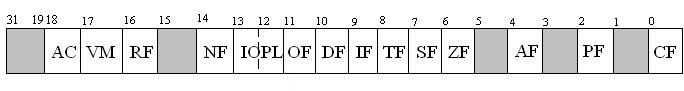
\includegraphics[scale = 0.5]{flags.jpg}
\end{figure}


\begin{enumerate}
\item CF "--- флаг переноса. Устанавливается в единицу, если при сложении происходит перенос за разрядную сетку, а при вычитании
требуется заём. 
\item FF "--- флаг четности. Устанавливается в единицу, если в младшем байте результата окажется четное количество единиц.
\item AF "--- флаг полупереноса. Устанавливается в единицу, если при сложении(вычитании) происходит перенос из третьего разряда
в четвертый(требуется заём из четвертого в третий)
\item ZF "--- флаг нуля. Устанавливается в единицу, если все разряды результата равны нулю.
\item SF "--- флаг знака. Всегда равен знаковому разряду результата. Положительный результат "--- ноль, отрицательный "--- единица.
\item TF "--- флаг трассировки. Установленный в единицу переводит процессор в режим пошагового выполнения программы.
\item IF "--- флаг прерывания. Установленный в единицу, позволяет остановить обработку некоторых прерываний.
\item DF "--- флаг направления. Определяет режим работы со строками. Если DF равен нулю, строка обрабатывается в сторону старших
адресов, в сторону младших в противном случае. При этом автоматически увеличивается(уменьшается) содержимое индексных регистров
если DF = 0 (DF = 1).
\item OF "--- флаг переполнения. Устанавливается в единицу, если результат превышает максимально допустимый для данной разрядной
сетки.
\item AC "--- флаг выравнивания операндов. Установленный в единицу, вызовет сообщение об ошибке, если адреса слов и двойных слов
не кратны двум или четырем соответственно.
\item VM "--- флаг виртуальных машин. Установленный в единицу, ползволяет перевести процессор в режим виртуальных машин.
\item RF "--- флаг маскирования прерывания. Позволяыет запретить прерывание.
\item NT "--- флаг вложенной задачи. Позволяет перейти в режим вложенной задачи.
\item IOPL "--- флаг уровня привелегий текущей программы. Если он окажется меньше значения флага, то программе будут запрещены
операции ввода/вывода.
\end{enumerate} 

\subsection{Оперативная память (RAM)}

Оперативная память состоит из байтов. Байт состоит из восьми информационных битов. Разряды с нулевого по третий "---
цифровая часть байта, с четвертого по седьмой "--- зонная часть байта.
\begin{figure}[H]
    \centering
    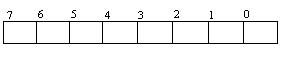
\includegraphics[scale = 0.5]{ram.jpg}
\end{figure}
32-х разрядный процессор может работать с оперативной памятью до 4 Гб, а значит физический адрес байта может изменяться от 
0 до $2^32 - 1$, что в Шестнадцатиричной системе записывается как $00000000 -> FFFFFFFF$.

Байты могут объединяться в поля фиксированной и переменной длины. Такие поля имеют собственные имена "--- слово (2 байта), двойное слово (4 байта).
Поле переменной длины может состоять из произвольного количества байтов. Адресом такого поля может быть адрес любого байта,
но это адрес младшего байта, входящего в поле.

Поле может использоваться как непрерывная память, либо сегментированная. В случае, если память сегментирована, то память
записывается как <сегмент>: <смещение>, а вычислено может быть по формуле ФА = АС + ИА, где АС - опредяется сегметным регистром,
а ИА "--- смещение сегмента, формируемое в команде и зависит от способа адрессации операнда.

В защищенном режиме программа может определять до 16383 сегментов размером до 4 Гб, и таким образом работать с 
64 ТБайтами виртуальной памяти.

Для реального режима адрес сегмента определяется сегментным регистром, и для получения 20-разрядного двоичного адреса
байта содержимое сегментного регистра, смещенного на 4 разряда влево прибавляют смещение (ИА).

\section{Работа с ассемблером}
\subsection{Форматы данных}

Процессор ix86 вместе с сопроцессором могут обрабатывать целые числа без знака, целые числа со знаком, действительные с плавающей
точкой, двоично-десятичные, символы, строки, указатели.
\paragraph{Целые числа.}

Целые двоичные без знака могут занимать байт, слово или двойное слово и принимать числа из диапазона 0-255, 0-65535, 0-4294967295
соответственно.
Целые числа со знаком так же могут занимать байт, слово или двойное слово, но представляются в дополнительном коде.

Дополнительнй код положительного числа совпадает с записью числа, а дополнительный код отрицательного числа может быть получен по
формуле $X = 10^n - |X|$.
Дополнительный код двоичного числа можно получить инверсией всех разрядов числа и добавление единицы к младшему разряду.

Вычитание в машине заменяется сложением уменьшаемого и доп. кодом вычитаемого числа. 
Действительные числа(числа с плавающей точкой) могут занимать 32 разряда (короткое), 64 разряда (длинное), 80 разрядов (рабочее).
Формат числа с плавающей точкой состоит из трех полей: знак числа, машинный порядок и мантисса.

Порядки:

$1 + 8 + 23 -> -10^{+-32} - 10^{+-32}$

$1 + 11 + 52$

$1 + 15+ 64$

Машинный порядок неявным образом включает в себя знак порядка. Он связан истинным следующим соотношением: $P_m = P_i + 127(1023, 16383)$.
Мантисса должна быть нормализованной, и старшая единица в разрядную сетку не помещается для экономии памяти.

\paragraph{Двоично"=десятичные числа.}

Процессор может обратаывать двоично"=десятичные числа в упакованном или неупакованном формате, а 
сопроцессором могут обрабатываться 90-ти разрядные данные в упакованном формате.

Они неупакованные "--- одну цифру в одной части байта.

\paragraph{Символы.}

Для символом используется кодировка ASCII. Для любого символа отводится один байт.
Строковые данные являются последовательностью байтов, слов или двойных слов.

Указатели на строку подразделяются на два типа:
длинный указатель, занимающий 48 бит (32 смещение + 16 сегмент)
короткий указатель, занимающий 32 бита(32 смещение)

\subsection{Форматы команд}

Команды "--- последовательность нулей или единиц, состоящих из двух подпоследовательностей.
Одна из них определяет код операции (сложить, умножить и т.~д), а другая определяет адреса операндов
и адрес размещения результата команды.

Операндами могут быть байтом, словом или двойным словом. Команда в свою очередь может быть безадресной, 
одноадресной, двухадресной или трехадресной.

В памяти команда может занимать от одного до 15 байтов, в зависимости от кода операции, количества и
размера операндов. Операнды могут находиться в команде, в регистрах или памяти. В одноадресной команде
операнд находится или в регистре, или в памяти, самое большое количество команд "--- двухадресные.

Существуют различные форматы двухадресных команд, которые отличаются расположением команд.
Регистр"=регистр, память"=память, регистр"=память, память"=регистр, данные"=память, память"=данные.

В общем случае, исполняемый адрес может состоять из трех частей: база, индекс и смещение.
Существуют различные способы способы адресации операндов, такие как:
\begin{enumerate}
    \item регистровая
    \item непосредственная
    \item прямая
    \item косвенно"=регистровая
    \item по базе со смещением
    \item прямая с индексированием
    \item по базе с индексированием (двумерные массивы)
    \item косвенная адресация с масштабированием
    \item базово"=индексная с масштабированием
    \item базово"=индексная с масштабированием и смещением
    
\end{enumerate}


\subsection{Примеры команд с различным способом адресации}

\begin{enumerate}
    \item Регистровая.
    \verb|mov AX, BX|
    \item Непосредственная.
    \verb|mov AX, 25|
    Кроме того, можно передать именованную константу с помощью конструкции \verb|const EQU 34h|
    \item Прямая. Если известен адрес в памяти, то в команде можно непосредственно передать этот адрес:
    \verb|mov AX, ES : 0001|, где ES "--- регистр сегмента данных, 0001 "--- смещение внутри сегмента. В таком случае
    содержимое двух байтов, начиная с адреса (ES) + 0001 пересылаются в AX
    ((ES) + 0001) -> AX

    Прямая адресация может быть записана с помощью символического имени, если этому имени
    предварительно поставить в соответствие некоторый адрес в оперативной памяти, а сделать
    это можно с помощью специальной директивы "--- директивы определения данных и памяти.
    
    DB "--- define byte
    DW "--- define word
    DD "--- define double word
    
    Если в сегменте ES содержится директива Var_p DW ?, тогда передадим по команде

    \verb|mov AX, ES: Var_p; ((ES) + Var_p) -> AX|
    \item Косвенно"=регистровая
    
    Данный вид адресации отличается от регистровой адресации тем, что в регистре содержится
    не сам операнд, а адрес области памяти, в которйо операнд содержится.
    
    \verb|mov AX,[SI]|
    
    Нельзя использовать AX, CX, DX, SP, ESP, остальные регистры допустимы.
    
    \item По базе со смещением

    \verb|mov AX, [BX] + 2; ((DS) + BX + 2)->AX|

    \verb|mov AX, [BP] + 4; ((SS) + (BP) + 4)->AX|
    
    \item Прямая с индексированием
    
    \verb|mov AX, MAS[SI]; ((DS) + (SI) + MAS)->AX|

    Эту адресацию используют с полями структуры. С двумерными массивами можно работать с адресацией по базе с индексированием.
    
    \item По базе с индексированием
    
    \verb|mov AX,Arr[BX][DI]; ((DS) + (BX) + (DI) + Arr)->AX|

    \item По базе с масштабированием
    
    \verb|MOVAX, [EBX*4]+2; Только для 32-х разрядных операндов|

Символическое имя определяет начало массива, с помощью базового регистра осуществляется
переход от одной строки к другой. Кроме того, используется при массивах структур.
   
\end{enumerate}

Особенности работы команд пересылки:
\begin{itemize}
    \item Нельзя пересылать из одной памяти в другую
    \item Нельзя пересылать информацию из одного сегментного регистра в другой.
    Если есть такая необходимость нужно воспользоваться регистром общего назначения или стеком
    для промежуточной пересылки.
    \item Нельзя пересылать непосредственный операнд в сегментный регистр. Если же такая
    необходимость есть "--- использовать регистр общего назначения.
    \item Нельзя командой mov изменять содержимое регистра CS.
    \item Данные в памяти хранятся в перевернутом виде, а в регистрах в нормальном
    виде, команда mov это учитывает.
    Например, R DW 1234h. Тогда в байте с адресом R будет 34h, а в байте R + 1 12h.
    Обратная картина в AH и AL при выполнении mov AX, R.
    \item Размер передаваемых данных определяется типом операнда.
    Например, пусть \verb|X DB ?, Y DW ?|, тогда при выполнении \verb|mov X, 0| в один байт запишется
    ноль, а если \verb|mov Y, 0| "--- два байта вместо одного.

    \verb|mov [SI], 0| "--- сообщение об ошибке. Чтобы этого не случилось, нужно определить
    тип операнда с помощью оператора PTR:

    \verb|<ТИП> PTR <ВЫРАЖЕНИЕ>|

    Выражение может быть как константным, так и адресным, а тип это: BYTE, WORD, DWORD и т.д.

    Например: \verb|mov Byte PTR[SI], 0| или \verb|mov [SI], byte PTR 0|.
    \item Если тип обоих операндов определен, известен, то эти типы должны соответствовать друг@=другу.
\end{itemize}

К командам пересылки относится команда \verb|xchg|. Операндами могут быть регистр"=регистр, регистр"=память.
Для перестановки значений байтов внутри регистра используют \verb|BSWOP|.

Также существуют команды конвертирования: \verb|CRW, CWD, CWE, CDF| (последние две для x386 и выше).

Есть команды условной пересылки: \verb|CMOVxx|.

Команда загрузки адреса: \verb|LEA OP1, OP2| "--- вычисляет адрес OP2 и пересылает первому операнду,
который может быть только регистром.

\subsection{Структура программы на ассемблере}

Программа на ассемблере должна пройти три этапа обработки.

На первом этапе, в процессе ассемблирования, исходный модуль преобразуется в машинный
код, таким образом получается объектный модуль исходных модулей и объектов может быть
несколько.

На втором этапе с помощью редактора связей (компоновщика) объектные модули преобразуются
в исполняемый модуль (\verb|.exe|, \verb|.com|). Для получения com"=файла нужно выполнить ещё один
этап обработки с помощью системной обрабатывающей программы. Для получения \verb|.com| файла
из \verb|.exe| файла нужно, чтобы исходный модуль удовлетворял определенным требованиям.

Исходный файл на ассемблере состоит из команд, директив и комментариев. Команды
в процессе ассемблирования преобразуются в программы на машинном языке, определяющим
этапы решения задачи. Директивы определяют форматы данных (исходных, промежуточных, окончательных)
и их размещение в памяти, а также определяют как программа должна быть транслирована ассемблером.

Команда в ассемблере в общем виде состоит из четырех полей:

\verb|[<имя>][:]<код операции>[<операнды>][комментарий]|

В скобках располагаются необязательные поля. Имя "--- символическое имя ассемблера, которое
используется как метка команды, на которую можно передать управление. Если после
имени стоит двоеточие, то такая метка называется внутренней и на нее можно передать
управление только из сегмента, в котором эта команда содержится.

Операнды отделяются друг от друга запятой, все поля отделяются друг от друга хотя бы
одним пробелом, а перед комментарием ещё записывается точка с запятой. Комментарий
может занимать часть строки или всю строку.
Например, \verb|JMP M1| "--- команда передачи управления на команду с меткой M1.

Директива, как и команда, состоит из четырех полей:

\verb|[<имя>]<код псевдооперации> <операнды> [; комментарий].|

Код псевдооперации  назначение директивы.
Операндов может быть различное количество в одной директиве.

\verb|M1 DB 1, 0, 1, 0, 1| "--- выделение пяти байтов подряд.

Proc "--- директива начала процедуры, endp "--- конца.

Исходный модуль на ассемблере состоит из последовательности строк, команд, директив и комментариев
и при ассемблировании текст просматривается сверху вниз слева направа от начала, пока
не увидит директиву end, которая и символизирует конец исходного текста программу.
Обычно программа состоит из трех сегментов. 

\begin{minted}{asm}
    Sseg Segment
    ...
    Sseg ends
    DSeg Segment
    ...
    DSeg ends
    CSeg Segment
    ...
    Cseg ends
    end start
\end{minted}

Каждый сегмент начинается с директивы Segment и заканчивается директивой ends. Параметры
директивы Segment говорят о назначении сегмента. Кроме того, в кодовом сегменте сразу
после директивы Segment должна располагаться директива, устанавливающая соответствие
между именами в директивах Segment и сегментными регистрами "--- \verb|assume|.

\begin{minted}{asm}
    assume SS :SSeg, CS: CSeg, DS: Dseg, ES: Dseg
\end{minted}

Кодовый сегмент выглядит как процедура, это может быть одна процедура или последовательность
процедур.

Структура кодового сегмента с использованием двух вложенных процедур выглядит следующим
образом:

\begin{minted}{asm}
    Cseg segment...
    assume...

    pr2 Proc
    ...
    pr2 ends

    pr1 Proc
    ...
    pr2
    pr1 ends

    end pr1
\end{minted}

В сегменте стека выделяется место под стек.
В сегменте данных определяются данные, используемые в программе, выделяется место
под промежуточные и окончательные результаты.
Кодовый сегмент содержит программу решения поставленной задачи.

\begin{minted}{asm}
    ;Prim1.asm
    ;Сегмент стека
    Sseg segment
        db 256 dup(?)
    Sseg ends
    ;Сегмент данных
    Dseg segment
        X db 'A'
        Y db 'B'
        Z db 'C'
    Dseg ends
    Cseg segment
        assume SS:Sseg, DS:DSeg, CS:Cseg
        start proc FAR
        push DS
        push AX
        mov DS, Dseg
        mov DS, DX
        call Main
        ret
    Start endp
    main proc NEAR
        add AL, X
        mov AX, Y
        ...
        ret
    main endp
    Cseg ends
    end start
\end{minted}

Наш кодовый сегмент представлен в виде двух последовательных процедур: первая из них
внешняя, об этом говорит параметр \verb|far| директивы \verb|Proc|, она реализует связь с операционной системой.
\verb|near| же говорит о том, что процедура внутренняя.

К внешней процедуре можно обратиться из любого кодового сегмента, к внутренней можно обратиться
только из того сегмента, в котором содержится её определение.

Программа на ассемблере может работать с целыми двоичными, десятичными, шестнадцатиричными, действительными
с плавающей точкой числами, символами и строками. Сигнатура двоичных чисел имеет вид <<xxxxb>>.

Десятичная константа записывается как обычное число, а шестнадцатиричная содержать <<h>> на конце,
если же ведущая цифра это А, B, C, D, E, F, то в начале необходимо поставить 0.

Двоичные числа имеют вид мантисса"=порядок. 

Пример: 34,751e+02. 

Строковые константы "--- последовательности символов,
заключенных апострофами или двойными кавычками.

Как и в языках высокого уровня, на ассемблере могут быть именованные или неименованные константы.
Примеры неименованных были рассмотрены выше, их тип и значение определяются внешним видом на этапе компиляции.
Именованные константы создает программист с помощью специальной директивы EQU. Пример: M EQU 27.
Символическому имени M присваивается константное значение 27.

Переменные в ассемблере определяются с помощью директивы определения данных и памяти: v1 DR ?
v2 DW 34 или с помощью знака равенства: v3 = 100. 
Константы обычно используются как непосредственный операнд и в директивах определения данных и памяти.

Выражения в ассемблере строятся из операндов, операторов и скобок. Операнды "--- константы и переменные,
операторы "--- знаки арифметических, логический, специальных операций, а также операций отношения.
Все арифметические, логические операции и операции отношения характерны и другим языкам. Среди специальных
операций выделяют offset и PTR. offset возвращает смещение переменной относительно начала сегмента.
PTR определяет один из следующих типов для операнда:
\begin{itemize}
    \item BYTE
    \item WORD
    \item DWORD
    \item FWORD
    \item QWORD
    \item TWORD  
\end{itemize}
Кроме того, к специальным операциям относят \verb|near| и \verb|far|.

\subsubsection{Директива определения.} 
Её синтаксис следующий:

\verb|[<имя>] D{X} <операнды>[<;комментарий>], где X "--- B, W, D, F, Q, T.|

Имя определяет адрес первого байта выделенного поля (если оно есть), операндом может быть знак вопроса
или константа. Если это константа, то она записывается в выделенное поле, если знак вопроса, то в выделенное поле не записывается ничего.

Если операндом является символоическое имя (пусть это будет \verb|IM1|), которому предварительно поставлено
в соответствие некоторое значение, например, \verb|03AC1h|, то после выполнения
\verb|M DD IM1| будет выделено 4 байта памяти, в которое запишется значение \verb|03AC1h|.

Для выделения большого количества памяти используются директива \verb|dup|, например \verb|D db 100 dup (1)|.
Аналогично определяется, например, одномерный массив слов, например \verb|mas dw 1, 7, 35, 75, 84|.
У двумерного массива хранится указатель на элемент нулевой строки, нулевого столбца.

\begin{minted}{asm}
    const EQU 100
    d db const dup (?)    
\end{minted}


C помощью директивы определения байта возможно определить константу максимальной допустимой величины 255, для слова "--- 65535.

С помощью директивы определения байта можно определить строковую константу до 255 символов

Команда прерывания.

Команда прерывания приостанавливает выполнение программы и передает выполнение операционной системе
или BIOS в зависимости от операнда этой команды, после чего выполняется системная обрабатывающая программа
и управление возвращается к следующей за ним. А какая системная обрабатывающая программа будет выполняться
зависит от содержимого некоторых регистров. Например: чтобы вывести на экран символ, нужно выполнить три команды:
\begin{minted}{asm}
    mov AH, 6
    mov DL, "!"
    int 21h    
\end{minted}
Стек определяется регистрами SS и SP(ESP).
Начало сегмента стека записывается в регистр SS автоматически, 
а указатель на вершину стека при добавлении элемента уменьшается на размер операнда, при удалении
"--- увеличивается. Чтобы добавить элемент в стек нужно вызвать функцию push, чтобы удалить "--- pop.

Для i186 существуют команды \verb|pusha| И \verb|popa|, которые позволяют загрузить и удалить последовательность регистров
AX, BX, DX, CX, SP, BP, SL, DL. С i386 есть команды pushad и popad "--- аналогичные команды для extended версий
регистров.

\begin{minted}{asm}
TITLE Pris.asm; заголовок листинга
Page, 120; длина
SSeg Segment Para stack 'stack'
DB 100h
SSeg ends

DSeg Segment Para Public 'Data'
DAN DB '1', '3', '5', '7'
REZ DB 4 DUP (?)
DSeg ends
;кодовый сегмент оформлен как одна внешняя процедура, к ней обращаются из отладчика

CSeg Segment Para Public 'Code'
ASSUME SS:SSeg, DS:DSeg, CS:CSeg; соответствие между сегментными регистрами и именами
start proc Far
push DSeg
xor AX, AX
push AX
mov AX, DSeg
mov DS,AX
mov AH, 6
mov DL, DAN + 3
mov REZ, DL
int 21h
mov DL, DAN + 2
mov REZ + 1, DL
int 21h
mov DL, DAN + 1
mov REZ + 2, DL
int 21h
mov DL, DAN
mov REZ + 3, DL
int 21h

mov AH, 4CH
int 21h
Start endp
CSeg ends
end Start
\end{minted}


\subsubsection{Директива сегмента.}

Общий вид:

\verb|<имя> Segment <ReadOnly> <Выравнивание> <тип> <размер> <'класс'>|.

\verb|ReadOnly| устанавливает режим только для чтения для этого сегмента.

Операнд <<выравнивание>> устанавливает адрес начала сегмента:
\verb|BYTE, WORD, DWORD| "--- кратность байту, двум или четырем соответственно.

\verb|Para| "--- кратность шестнадцати. \verb|Page| "--- кратность 256.

<<Тип>> определяет тип объединения сегментов. Для стека устанавливается stack, для остальных сегментов public.
Если этот параметр присутствует, то все сегменты с одним именем и различными кклассами объединяются в один
последовательно в порядке их записи.

Значение 'Common' говорит, что сегменты с одним именем объединены, но не последовательно, а с одного и того же
адреса так, что общий размер сегмента равен не сумме, а максимальному из них.

Значение \verb|IT <выражение>| означает, что сегмент должен быть расположен по абсолютному адресу, определяемым выражением.
'Private' говорит о том, что этот сегмент не объединяется ни с каким другим.

Параметр размер может принимать значения \verb|use 16|, \verb|use 32|.
\subsubsection{Точечные директивы.}

В программе на ассемблере могут использоваться точечные директивы:
.MODEL "--- директива, определяющая модель выделяемой памяти для программы.
МОдель памяти определяется параметром:
tiny "--- под всю программу выделяется 1 сегмент памяти.
small "--- под данный и под программу выделяются по одному сегменту.
medium "--- под данные выделяется один сегмент, под программу выделяется несколько сегментов.
compact "--- под программу выделяется один сегмент, под данные выделяется несколько сегментов.
large "--- под данные и под программу выделяются по n элементов.
huge "--- позволяет использовать сегментов больше, чем позволяет оперативная память.

\begin{minted}{asm}
    .model small
    .stack 100h
    .data 
    \dots
    .code
    begin:
    mov AX, @data
    mov ds, AX
    mov AH, 9
    mov DX, offset St1
    int 21h
    аналогично для остальных двух
    mov AH, 4CH
    int 21
    end begin    
\end{minted}

\subsubsection{COM"=файлы}

Результатом ассемблирования и редактора"=компоновщника является исполняемый exe"=файл, которые содержит в себе,
так называемый, блок начала загрузки размером в 512 байт.

Но ассемблер позволяет создать другой тип исполняемых
файлов \verb|.com|, который может быть получен на основе \verb|.exe| файла в результате его обработки системной программой
\verb|EXE2bin.com| или с помощью специального ключа в среде разработки. 
Не из всякого EXE"=файла можно создать
COM"=файл "--- исходный файл должен удовлетворять определенным требованиям.

\paragraph{Основные отличия}
\begin{itemize}
    \item COM"=файл не содержит блока начальной загрузки(512 байт)
    \item EXE"=файл занимает произвольный объем ОП, COM"=файл только один сегмент памяти.
    \item в COM"=файле стек создается автоматически ОС, поэтому у пользователя нет необходимости выделять для него место.
    \item В COM"=файле данные располагаются там же, где и программа. Т.к вся программа содержится в одном сегменте, все сегментые регистры содержать
    в качестве значения адрес префикса программного сегмента (psp). И т.к PSP содержит 256 байт, то ддя обхода этого блока применяется org 100h.
\end{itemize})

\subsubsection{Арифметические операции}

\paragraph{Сложение и вычитание}
Сложение(вычитание) беззнаковых чисел выполняется по правилам аналогичным сложению (вычитанию)
по модулю $2^k$, принятым в математике. Если в результате более $k$ разрядов, то $k+1$"=ый пересылается
в \verb|CF|.

То есть:
\begin{equation*}
    \begin{cases}
        X + Y = (X + Y) \text{mod} ~2^k = X + Y, ~\text{CF} = 0 & \text{если $X + Y < 2^k$} \\
        X + Y = (X + Y) \text{mod} ~2^k = X + Y, ~\text{CF} = 1 & \text{если $X + Y \ge 2^k$} \\

    \end{cases}    
\end{equation*}

Пример:
\begin{equation*}
    250 + 10 = (250 + 10) ~\text{mod}~ 2^8 = 260~ \text{mod} ~256 = 4
\end{equation*}

Сложение (вычитание) знаковых чисел сводится к сложению (вычитанию) с использованием дополнительного кода.

Например, $-1 = 256 - 1 = 255 = {11111111}_2$, $-3 = 256 - 3 = 253 = {11111101}_2$
\begin{equation*}
    3 - 1 = 3 + (-1) = (3 + (-1))~\text{mod}~256 = (3 + 255)~ \text{mod}~256 = 2
\end{equation*}

Ответ получили в дополнительном коде, следовательно результат получаем  в байте по формуле $X = 10^8 - |X|$, т.~е.
$X = 256 - 254 = |2|$ и знак минус. Ответ: -2.

Переполнение разрядной сетки происходит если есть перенос из старшего цифрового в знаковый, а из знакового нет, и
наоборот, тогда OF = 1. Программист сам решает какой флажок анализировать "--- OF или CF, зная 
с какими данными он работает.

\paragraph{Сложение и вычитание в Ассемблере}

Арифметические операции изменяют значение флажков OF, CF, SF, ZF, AF, IF.

В Ассемблере операция сложения представлена несколькими командами.

\begin{minted}{asm}
    add OP1, OP2; (OP1) + (OP2) -> OP1
    adc OP1, OP2; (OP1) + (OP2) + (CF) -> OP1
    xadd OP1, OP2; (OP1)<->(OP2), (OP1) + (OP2) -> OP1
    inc OP1; OP1 + 1 -> OP1
\end{minted}

Аналогично работают команды sub, sbb, dec. В командах сложения (вычитания) можно использовать любые способы адресации.

\paragraph{Умножение и деление}

Умножение беззнаковых чисел представлено командой MUL.
\begin{minted}{asm}
    MUL OP2; (OP)*(AL) or (AX) or (EAX) -> AX or DX:AX or EDX:EAX
\end{minted}

Умножение знаковых чисел определяется аналогичным образом, но с помощью команды IMUL.




К командам побитовой обработки данных относятся логические команды, команды сдвига, установки, сброса и инверсии битов.

К логическим операциям относят команды and, or, xor, not. Для всех логических команд, кроме not операнды одновременно
не могут находится в памяти. OF = CF = 0, AF - не определен, SF, ZF, PF определяются результатом команды.

Второй операнд называют маской. Основным назначением команды and является установка в ноль с помощью маски
некоторых разрядов первого операнда. 

\subsubsection{Директивы внешних ссылок}

Директивы внешних ссылок позволяют организовать связь между различными модулями и файлами, расположенными на диске.

\begin{minted}{asm}
    Public <имя> [,<имя>, ..., <имя>]
\end{minted}

определяет указанные имена как глобальные аеличины, к которым можно обратиться из других модулей. Имена здесь "---
имена меток и переменных, определенных с помощью директивы '=' и EQU.

Если некоторое имя определено в модуле A как глобальное, и к нему можно обратиться из других модулей B и C, то в этих
модулях должна быть директива вида

\begin{minted}{asm}
    EXTRN <имя>:<тип> [,<имя>:<тип>]
\end{minted}
Здесь имя то же, что и в \textbf{Public}, а тип определяется
следующим образом: если <имя> "--- это имя переменной, то типом
может быть: BYTE, WORD, DWORD, FWORD, QWORD, TWORD.
Если <имя> "--- это имя метки, то типом может быть \textbf{NEAR} и \textbf{FAR}.

Директива \textbf{EXTRN} говорит о том, что перечисленные имена являются
внешними для данного модуля.

\subsubsection{Команды управления}




\end{document}